\section{DeepSmith: Compiler Fuzzing Through Deep Learning}
\label{sec:deepsmith}

DeepSmith is an open source framework for compiler fuzzing. Figure~\ref{fig:deepsmith} provides a high-level overview. This section describes the three key components: a generative model for random programs, a test harness, and voting heuristics for differential testing.

\begin{figure}
  \centering
  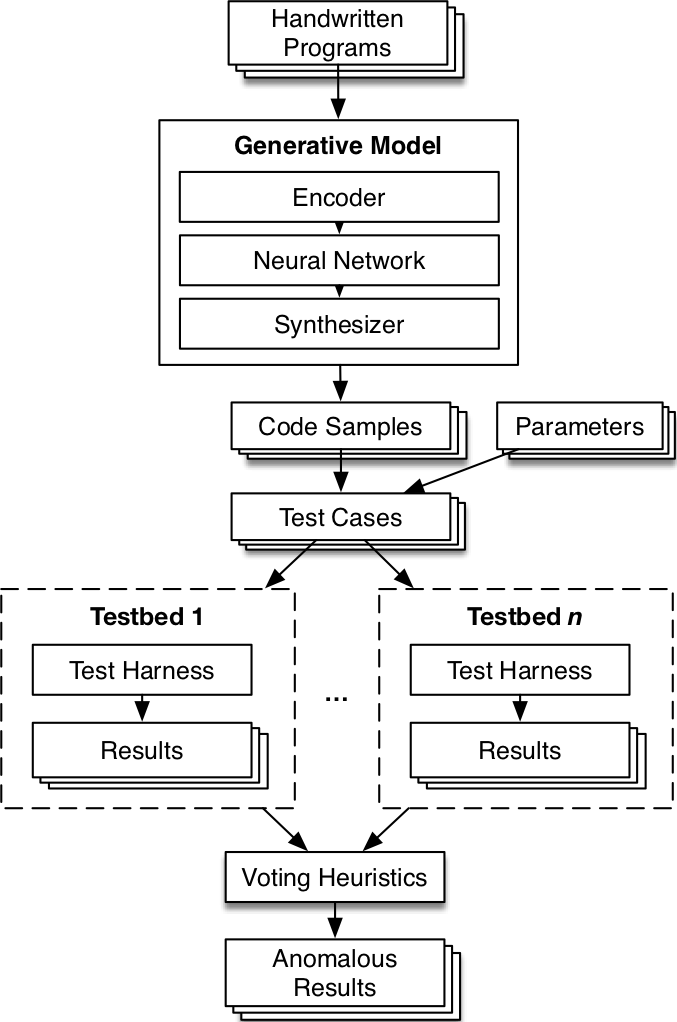
\includegraphics[width=.7\columnwidth]{img/deepsmith}
  \caption[DeepSmith system overview]{%
    DeepSmith system overview. \diff{Handwritten programs are used to derive a generative model; from which code samples are produced and parameterised to make test cases. Test cases are broadcast to multiple testbeds, and voting heuristics used to determine the testbeds that deviate from the majority, exposing anomalous results.}
  }%
  \label{fig:deepsmith}
\end{figure}

\subsection{Generative Model}

Generating test cases for compilers is hard because their inputs are highly structured. Producing text with the right structure requires expert knowledge and a significant engineering effort, which has to be repeated from scratch for each new language. Instead, the proposed approach frames the problem as an unsupervised machine learning task, extending prior work of Chapter~\ref{chap:clgen} in employing state-of-the-art deep learning techniques to build models for how humans write programs. The approach is inspired by breakthrough results in modelling challenging and high dimensional data sets through unsupervised learning~\cite{Raghu2016,Radford2016b,Bowman2015}. Contrary to existing tools, this approach does not require expert knowledge of the target language and is only a few hundred lines of code.

\paragraph*{Handwritten Programs}

The generative model needs to be trained on a \emph{seed corpus} of example programs. The assembly of this corpus is automated by mining 10k OpenCL kernels from open source repositories on GitHub. An \emph{oracle compiler} (LLVM 3.9) is used to statically check each downloaded source file, discarding files that are not well-formed. The main purpose of this step is to remove the need to manually check that each file selected from GitHub does indeed contain OpenCL. A downside is that any training candidate which triggers a bug in the LLVM 3.9's front end will not be included. However, this did not prevent our system from uncovering errors in that compiler (Section~\ref{subsec:clangs}).

This corpus, exceeding one million lines of code, is used as a representative sample of OpenCL code from which a generative model can be derived.

As in Chapter~\ref{chap:clgen}, semantic-preserving transformations are employed to simplify the training programs. First, each source file is preprocessed to expand macros and remove conditional compilation and comments. Then, all user-declared identifiers are renamed using an arbitrary, but consistent pattern based on their order of declaration: $\{a,\allowbreak b,\allowbreak c,\allowbreak \ldots,\allowbreak aa,\allowbreak ab,\allowbreak ac,\allowbreak \ldots\}$ for variables and $\{A,\allowbreak B,\allowbreak C,\allowbreak \ldots,\allowbreak AA,\allowbreak AB,\allowbreak AC,\allowbreak \ldots\}$ for functions. This ensures a consistent naming convention, without modifying program behaviour. Finally, a uniform code style is enforced to ensure consistent use of braces, parentheses, and white space. These rewriting simplifications give more opportunities for the model to learn the structure and deeper aspects of the language and speed up the learning. On the other hand, some bugs in the preprocessor or front-end might no longer be discoverable. For the purpose of fuzzing OpenCL compilers, this was reasoned as an acceptable trade-off. For languages where the corpus can be many orders of magnitude larger, for example, C or Java, it may be possible to construct effective models without these modifications.


\paragraph*{Encoder}

Source code is encoded as a sequence of integers for interpretation by artificial neural networks, where each integer is an index into a predetermined vocabulary. In~\cite{Jozefowicz2016a}, a character based vocabulary is used. This minimises the size of the vocabulary but leads to long sequences which are harder to extract structure from. In~\cite{Allamanis2013a}, a token based vocabulary is used. This leads to shorter sequences, but causes an explosion in the vocabulary size, as every identifier and literal must be represented uniquely.

A hybrid, partially tokenised vocabulary approach is used. This allows common multi-character sequences such as \texttt{float} and \texttt{if} to be represented as unique vocabulary items, while literals and other infrequently used words are encoded at the character level.

First, a candidate vocabulary $V_c$ is assembled for the OpenCL programming language containing the 208 data types, keywords, and language builtins of the OpenCL programming language. From this, the subset of the candidate vocabulary $V \in V_c$ which is required to encode a corpus of 45k lines of GPGPU benchmark suite kernels is derived. Beginning with the first character in the corpus, the algorithm consumes the longest matching sequence from the candidate vocabulary. This process continues until every character in the corpus has been consumed, illustrated in Algorithm~\ref{alg:maxmunch-tokenization}. The resulting derived vocabulary consists of 128 symbols which we use to encode new program sources.

\begin{algorithm}
  \begin{algorithmic}[1]
\Require Candidate vocabulary $V_c$, string $S$.
\Ensure Vocabulary $V$.
\State $V \gets \varnothing$\algorithmiccomment{Initialise empty derived vocabulary}
\State $i \gets 1$
\While{$S \ne ``''$}\algorithmiccomment{While input not fully processed}
  \State $i \gets i + 1$\algorithmiccomment{Advance to next character}
  \State $c \gets [S^{(1)}, \ldots, S^{(i)}]$\algorithmiccomment{Read token from input}
    \If{$! IsValidPrefix(c, V_c)$}\algorithmiccomment{If token is not legal}
      \State $c \gets FindLongestSubstring(c, V_c)$\algorithmiccomment{Revert to last legal token}
      \State $S \gets [S^{(|c|)}, \ldots, S^{(|S|)}]$\algorithmiccomment{Pop token from input}
      \State $V \gets V \cup \{ c \}$\algorithmiccomment{Add token to vocabulary}
    \State $i \gets 1$
  \EndIf
\EndWhile
\end{algorithmic}

  \caption[Deriving a vocabulary from a string]{%
    \diff{Deriving a hybrid token- and character-level vocabulary from a string.}%
  }
  \label{alg:maxmunch-tokenization}
\end{algorithm}

\paragraph*{Neural Network}

The Long Short-Term Memory (LSTM) architecture of Recurrent Neural Network is used to model program code~\cite{Hochreiter1997}. In the LSTM architecture activations are learned with respect not just to their current inputs but to previous inputs in a sequence. In our case, this allows modelling the probability of a token appearing in the text given a history of previously seen tokens. Unlike previous recurrent networks, LSTMs employ a \emph{forget gate} with a linear activation function, allowing them to avoid the \emph{vanishing gradients} problem~\cite{Pacanu2013}. This makes them effective at learning complex relationships over long sequences~\cite{Lipton2015} which is important for modelling program code. Extending the character-based model of Chapter~\ref{chap:clgen}, LSTM networks are employed to model the token-vocabulary distribution over the encoded corpus.

Compared to prior character-based models, the hybrid token vocabulary caused models to respond differently to model parameters. Initial experiments using different model parameters revealed that a two-layer LSTM network of 512 nodes per layer provided a good trade-off between the fidelity of the learned distribution and the size of the network, which limits the rate of training and inference. The network is trained using Stochastic Gradient Descent for 50 epochs, with an initial learning rate of 0.002 and decaying by 5\% every epoch. Training the model on the OpenCL corpus took 12 hours using a single NVIDIA Tesla P40. The model is given no prior knowledge of the structure or syntax of a programming language.

\paragraph*{Program Generation}

The trained network is sampled to generate new programs. The model is seeded with the start of a kernel (identified in OpenCL using the keywords \texttt{kernel void}) and sampled token-by-token. A ``bracket depth'' counter is incremented or decremented upon production of \texttt{\{} or \texttt{\}} tokens respectively so that the end of the kernel can be detected and sampling halted. Unlike in Chapter~\ref{chap:clgen}, there is no support for forcing kernel specifications, and there is no upper bound on the length of a sample. The generated sequence of tokens is then decoded back to text and used for compiler testing.


\subsection{Test Harness\label{sec:test-harness}}

OpenCL is an embedded compute kernel language, requiring host code to compile, execute, and transfer data between the host and device. For the purpose of compiler fuzzing, this requires a \emph{test harness} to run the generated OpenCL programs. At first, the test harness of CLSmith was used. The harness assumes a kernel with no input and a \texttt{ulong} buffer as its single argument where the result is written. Only 0.2\% of the GitHub kernels share this structure. A more flexible harness was desired so as to test a more expressive range of programs, capable of supporting multi-argument kernels and generating data to use as inputs.

A new harness was developed, extending CLdrive, which first determines the expected arguments from the function prototype and generates host data for them. At the moment, scalars and arrays of all OpenCL primitive and vector types are supported. For a kernel execution across $n$ threads, buffers of size $n$ are allocated for pointer arguments and populated with values {$[1 \ldots n]$}; scalar inputs are given value $n$ since scalar integer arguments are frequently used in OpenCL for specifying buffer sizes.

The training programs from which the generative model is created are real programs, and as such do not share the argument type restrictions. The model, therefore, may generate correct programs for which the driver cannot create example inputs. In this case, a ``compile-only'' stub is used, which only compiles the kernel, without generating input data or executing the compiled kernel.

Unlike the generative model, this test harness is language-specific and the design stems from domain knowledge. Still, it is a relatively simple procedure, consisting of a few hundred lines of Python.

\paragraph*{Test Harness Output Classes}

Executing a test case on a testbed leads to one of seven possible outcomes, illustrated in Figure~\ref{fig:test-process}. A \emph{build failure} occurs when the online compilation of an OpenCL kernel fails, usually accompanied by an error diagnostic. A \emph{build crash} or \emph{build timeout} outcome occurs if the compiler crashes or fails to produce a binary within 60 seconds, respectively. For compile-only test cases, a \emph{pass} is achieved if the compiler produces a binary. For test cases in which the kernel is executed, kernel execution leads to one of three potential outcomes: \emph{runtime crash} if the program crashes, \emph{timeout} if the kernel fails to terminate within 60 seconds, or \emph{pass} if the kernel terminates gracefully and computes an output.

\begin{figure}
  \centering %
  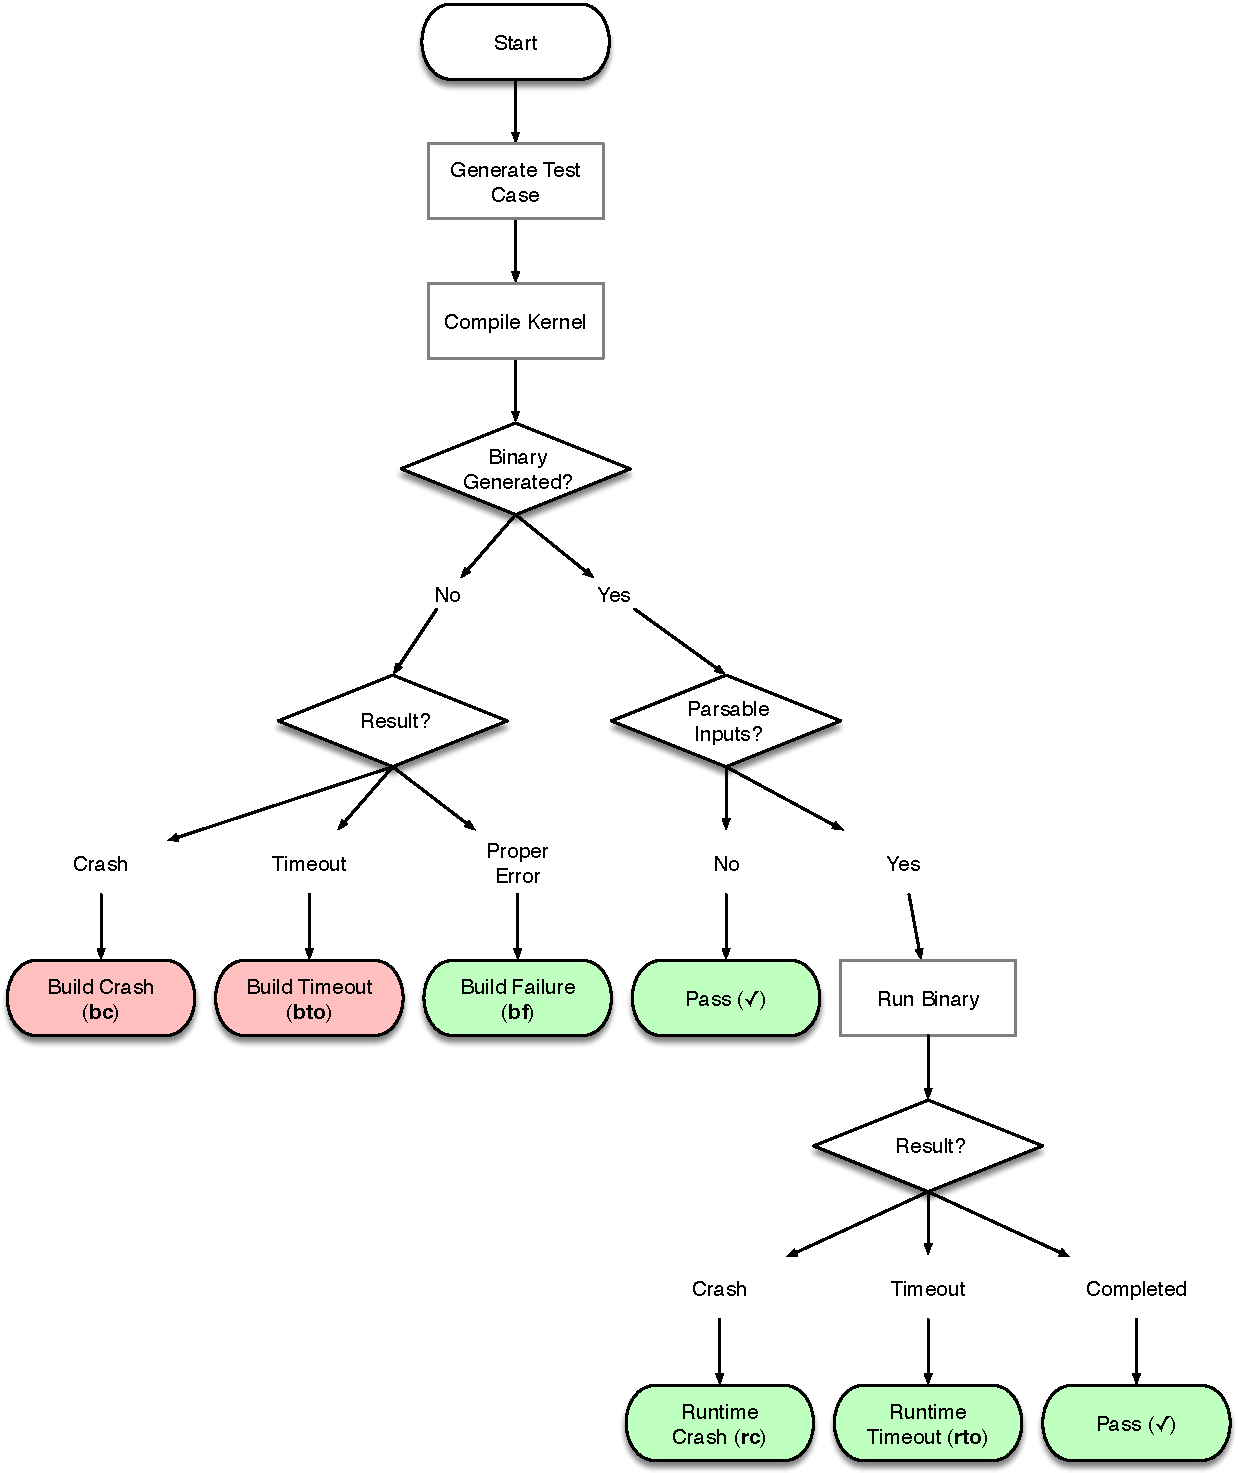
\includegraphics[width=\columnwidth]{img/testcase-flow-chart}
  \caption[Test case execution, and possible results]{%
    Test case execution, and possible results. \diff{Generating and executing a test case leads to one of six possible outcomes. Of these, build crashes and build timeouts are considered errors. In the remaining four cases, differential testing may be used to determine if the outcome is anomalous.}%
  }%
  \label{fig:test-process}
\end{figure}


\subsection{Voting Heuristics for Differential Testing}

Established Differential Testing methodologies are employed to expose compiler defects. As in prior work, voting on the output of programs across compilers has been used to circumvent the \emph{oracle problem} and detect miscompilations~\cite{McKeeman1998}. However, this approach is extended to describe not only miscompilations, but also anomalous build failures and crashes.

When evaluating the outcomes of test cases, build crash (\bc) and build timeout (\bto) outcomes are of immediate interest, indicative of erroneous compiler behaviour (examples may be found in Section~\ref{subsec:compile-time-defects}). For all other outcomes, \emph{differential tests} are required to confirm anomalous behaviour. The idea is to identify test cases where there is a majority outcome -- i.e. for which some fraction of the testbeds behaves the same -- but some testbed deviates. The presence of the majority increases the likelihood that there is a `correct' behaviour for the test case. In this work, a majority fraction of $\ceil{\frac{2}{3}n}$ is used, where $n$ is the number of testbeds.

An \emph{anomalous build failure} (\abf) or \emph{anomalous runtime crash} (\arc) occurs if, for a given test case, the majority of testbeds execute successfully, and a testbed yields a compilation error or runtime crash. An \emph{anomalous wrong-output} (\awo) occurs if, for a given test case, the majority of testbeds execute successfully, producing the same output values, and a testbed yields a result which differs from this majority output. Anomalous wrong-output results are indicative of \emph{miscompilations}, a particularly hard to detect class of bug in which the compiler silently emits wrong code. CSmith is designed specifically to target this class of bug.

\paragraph*{False Positives for Anomalous Runtime Behaviour}

Generated programs may contain undefined or non-deterministic behaviour which will incorrectly be labelled as anomalous. CSmith circumvents this problem by performing complex analyses during generation so as to minimise the chance of producing programs with undefined behaviour. Although similar analyses could be created as filters for DeepSmith, a simpler approach is taken, filtering only the few types of non-deterministic behaviour that have been actually observed to happen in practice.

Data races, out-of-bounds and uninitialised accesses are filtered using GPUverify~\cite{Betts2012} and Oclgrind~\cite{Price2015}. Some compiler warnings provide a strong indication of non-deterministic behaviour (e.g. comparison between pointer and integer) -- these warnings are checked for and filtered accordingly.

Floating point operations in OpenCL can be imprecise, so kernels can produce different output on different testbeds. For this reason, CSmith and CLSmith do not support floating point operations. DeepSmith permits floating point operations but since it cannot apply differential testing on the outputs, it can detect all results except for the \emph{anomalous wrong-output} results.

The last type of undefined behaviour observed comes from division by zero and related mathematical functions which require non-zero values. A simple detection and filtering heuristic was applied -- the input values are changed and the output is checked to see if it remains anomalous. While theoretically insufficient, in practice no false positives have been found to remain.
